\documentclass[aspectratio=169, 10pt]{beamer}

\usepackage{bm} % bold math
\usepackage{fontspec}
\usepackage{minted}
\usepackage{pgf-pie}
\usepackage{tikz}

% Custom commands and environments
\makeatletter
\newcommand\version[1]{\renewcommand\@version{#1}}
\newcommand\@version{}
\def\insertversion{\@version}

\newcommand\course[1]{\renewcommand\@course{#1}}
\newcommand\@course{}
\def\insertcourse{\@course}

\newcommand\coursetitle[1]{\renewcommand\@coursetitle{#1}}
\newcommand\@coursetitle{}
\def\insertcoursetitle{\@coursetitle}

\newcommand\lecturenumber[1]{\renewcommand\@lecturenumber{#1}}
\newcommand\@lecturenumber{}
\def\insertlecturenumber{\@lecturenumber}
\makeatother

\newcommand{\slidetitle}[1]{{\xbseries \large \structure{#1}} \bigskip}
\newcommand{\term}[1]{{\color{blue} #1}}
\newcommand{\leftspace}{\hspace{1em}}
\newcommand{\inlinearrow}{
  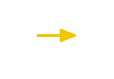
\begin{tikzpicture}[baseline]
    \node [anchor=base] (x) {};
    \draw [rawarrow] (x.mid west) -- ($(x.mid west) + (2em,0)$);
  \end{tikzpicture}
}

\newenvironment{slide}
{\begin{frame}[fragile,environment=slide]\vskip0pt plus 1filll}
{\vskip0pt plus 1filll\end{frame}}

% LaTeX

\setlength{\leftmargini}{1em}

% Common Information

\author{Jon Eyolfson}
\course{ECE 353}
\coursetitle{Systems Software}
\date{2024 Winter}

% fontspec

\defaultfontfeatures{Ligatures=TeX}
% \setmainfont{Domine}
\setsansfont{Inter}[
  FontFace={ul}{n}{Font=*-Thin},
  FontFace={el}{n}{Font=*-ExtraLight},
  FontFace={l}{n}{Font=*-Light},
  FontFace={sb}{n}{Font=*-SemiBold},
  FontFace={eb}{n}{Font=*-ExtraBold},
  FontFace={xb}{n}{Font=*-Black},
]
\setmonofont[Contextuals=AlternateOff, Ligatures=TeXOff]{Iosevka}[
  FontFace={xb}{n}{Font=*-Heavy},
]

%% Font Weights

\DeclareRobustCommand{\ulseries}{\fontseries{ul}\selectfont}
\DeclareTextFontCommand{\textul}{\ulseries}
\DeclareRobustCommand{\elseries}{\fontseries{el}\selectfont}
\DeclareTextFontCommand{\textel}{\elseries}
\DeclareRobustCommand{\lseries}{\fontseries{l}\selectfont}
\DeclareTextFontCommand{\textl}{\lseries}
\DeclareRobustCommand{\sbseries}{\fontseries{sb}\selectfont}
\DeclareTextFontCommand{\textsb}{\sbseries}
\DeclareRobustCommand{\ebseries}{\fontseries{eb}\selectfont}
\DeclareTextFontCommand{\texteb}{\ebseries}
\DeclareRobustCommand{\xbseries}{\fontseries{xb}\selectfont}
\DeclareTextFontCommand{\textxb}{\xbseries}

% tikz

\usetikzlibrary{
  arrows,
  arrows.meta,
  automata,
  backgrounds,
  calc,
  decorations.pathreplacing,
  matrix,
  positioning,
  overlay-beamer-styles,
  shapes,
  shapes.multipart,
  tikzmark,
}

\tikzstyle{rawarrow} = [
  -{Latex[round]},
  line width=1pt,
  yellow,
  shorten >=3pt,
  shorten <=3pt,
  font=\small,
  text=black,
]

\tikzstyle{arrow} = [
  -{Latex[round]},
  line width=1pt,
  yellow,
  shorten >=3pt,
  shorten <=3pt,
  transform canvas={yshift=3pt},
  font=\small,
  text=black,
]

\newcommand{\tikzmarkcoord}[1]{([yshift=3pt]pic cs:#1)}

% minted

\setminted{style=eyolfson, fontsize=\small, escapeinside=||}
\setmintedinline{fontsize=\normalsize}

% hyperref

\hypersetup{colorlinks, urlcolor=blue}

% beamer
\setbeamersize{text margin left=16mm, text margin right=16mm}
\setbeamertemplate{itemize items}[circle]
\setbeamercolor{item}{fg=black}
\setbeamercolor{structure}{fg=darkblue}
\setbeamerfont{frametitle}{series=\bfseries, parent=structure}
\setbeamertemplate{navigation symbols}{}
\setbeamertemplate{headline}{}
\setbeamertemplate{footline}{
  \begin{tikzpicture}[
    remember picture,
    overlay,
    shift={(current page.south west)},
  ]
    \path [fill=gray] (144mm, 0) -- (160mm, 16mm) -- (160mm, 0);
    \node [inner sep=3.5mm, outer sep=0, text=black, anchor=base east,
           align=right, yshift=3.5mm]
          at (current page.south east) {\ttfamily \small \insertframenumber{}};
  \end{tikzpicture}
}
\setbeamertemplate{title page}{
  \begin{tikzpicture}[
    remember picture,
    overlay,
    shift={(current page.south west)},
    background rectangle/.style={fill=darkblue},
    show background rectangle,
  ]
    \node [anchor=center, align=center, text=white, text width=40mm, scale=3.2]
          at (\paperwidth / 2, \paperheight * 2 / 3)
          {\xbseries \inserttitle{}};
    \node [anchor=base west, align=left, inner sep=0, text=white, yshift=2.5mm]
          at (16mm, \paperheight / 3)
          {\insertdate{} \insertcourse{}: \insertcoursetitle{}};
    \node [anchor=base west, align=left, inner sep=0, text=white, yshift=-2.5mm]
          at (16mm, \paperheight / 3)
          {\insertauthor};
    \node [anchor=base east, align=right, inner sep=0, text=white, yshift=2.5mm]
          at (144mm, \paperheight / 3)
          {Lecture \insertlecturenumber{}};
    \node [anchor=base east, align=right, inner sep=0, text=white,
           yshift=-2.5mm]
          at (144mm, \paperheight / 3)
          {\ttfamily \insertversion{}};
    \node [align=center, anchor=south, inner sep=0, text=white, yshift=3.5mm]
          (license) at (\paperwidth / 2, 0)
          {\fontsize{7pt}{7pt}\selectfont This  work is licensed under a
           \href{http://creativecommons.org/licenses/by-sa/4.0/}
                {\color{lightblue} Creative Commons Attribution-ShareAlike 4.0
                 International License}};
  \end{tikzpicture}
}

% xcolor

%% Primary Colour

\definecolor{pantone655}{RGB}{0, 42, 92} % #002a5c
\colorlet{darkblue}{pantone655}

%% Secondary Colours

\definecolor{pantone633}{RGB}{0, 139, 176} % #008bb0
\colorlet{blue}{pantone633}

\definecolor{pantonewarmred}{RGB}{220, 70, 51} % #dc4633
\colorlet{red}{pantonewarmred}

\definecolor{pantone3285}{RGB}{0, 161, 137} % #00a189
\colorlet{cyan}{pantone3285}

\definecolor{pantone7722}{RGB}{13, 83, 77} % #0d534d
\colorlet{darkcyan}{pantone7722}

\definecolor{pantone376}{RGB}{141, 191, 46} % #8dbf2e
\colorlet{green}{pantone376}

\definecolor{pantone2613}{RGB}{109, 36, 122} % #6d247a
\colorlet{violet}{pantone2613}

\definecolor{pantone2985}{RGB}{111, 199, 234} % #6fc7ea
\colorlet{lightblue}{pantone2985}

\definecolor{pantone227}{RGB}{171, 19, 104} % #ab1368
\colorlet{magenta}{pantone227}

\definecolor{pantone7406}{RGB}{241, 197, 0} % #f1c500
\colorlet{yellow}{pantone7406}

%% Neutrals

\definecolor{pantonecoolgray2}{RGB}{208, 209, 201} % #d0d1c9
\colorlet{gray}{pantonecoolgray2}


\lecturenumber{32}
\title{Buddy and Slab Allocators}
\version{2.0.0}

\begin{document}

  \begin{frame}[plain, noframenumbering]
    \titlepage
  \end{frame}

  \begin{slide}

    \slidetitle{The Buddy Allocator Restricts the Problem}

    Typically, allocation requests are of size $\mathsf{2^n}$

    \leftspace{}e.g. 2, 4, 8, 16, 32, ..., 4096, ...
    \medskip

    Restrict allocations to be powers of 2 to enable a more efficient
    implementation

    \leftspace{}Split blocks into 2 until you can handle the request
    \medskip

    We want to be able to do fast searching and merging

  \end{slide}

  \begin{slide}

    \slidetitle{You Can Implement the Buddy Allocator Using Multiple Lists}

    We restrict the requests to be $\mathsf{2^k, 0 \leq k \leq N}$ (round up if
    needed)
    \medskip

    Our implementation would use $\mathsf{N+1}$ free lists of blocks for each
    size
    \medskip

    For a request of size $\mathsf{2^k}$, search the free list until we find
    a big enough block

    \leftspace{}Search $\mathsf{k, k+1, k+2, ...}$ until we find one

    \leftspace{}\leftspace{}Recursively divide the block if needed until it's
    the correct size

    \leftspace{}\leftspace{}Insert “buddy” blocks into free lists
    \medskip

    For deallocations, we coalesce the buddy blocks back together

    \leftspace{}Recursively coalesce the blocks if needed

  \end{slide}

  \begin{slide}
    
    \slidetitle{Using the Buddy Allocator (1)}

    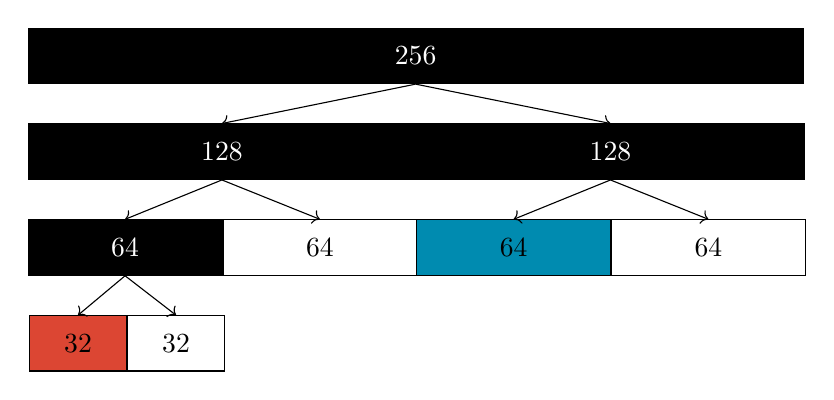
\begin{tikzpicture}[node distance=5mm and 0mm]
            
        \node[draw,rectangle,minimum width=280,minimum height=20,fill=black,text=white]    (a00)        {256};
        \node[draw,rectangle,minimum width=140,minimum height=20,fill=black,text=white,xshift=-70]    (a10) [below=of a00]       {128};
        \node[draw,rectangle,minimum width=140,minimum height=20,fill=black,text=white]    (a11) [right=of a10]       {128};
        \node[draw,rectangle,minimum width=70,minimum height=20,fill=black,text=white,xshift=-35]    (a20) [below=of a10]       {64};
        \node[draw,rectangle,minimum width=70,minimum height=20]    (a21) [right=of a20]       {64};
        \node[draw,rectangle,minimum width=70,minimum height=20,fill=pantone633,xshift=-35]    (a22) [below=of a11]       {64};
        \node[draw,rectangle,minimum width=70,minimum height=20]    (a23) [right=of a22]       {64};
        \node[draw,rectangle,minimum width=35,minimum height=20,fill=pantonewarmred,xshift=-17]    (a30) [below=of a20]       {32};
        \node[draw,rectangle,minimum width=35,minimum height=20]    (a31) [right=of a30]       {32};

        \draw[->] (a00.south) -- (a10.north);
        \draw[->] (a00.south) -- (a11.north);
        \draw[->] (a10.south) -- (a20.north);
        \draw[->] (a10.south) -- (a21.north);
        \draw[->] (a11.south) -- (a22.north);
        \draw[->] (a11.south) -- (a23.north);
        \draw[->] (a20.south) -- (a30.north);
        \draw[->] (a20.south) -- (a31.north);

    \end{tikzpicture}
    \medskip

    Where do we allocate a request of size 28?

  \end{slide}

  \begin{slide}
    
    \slidetitle{Using the Buddy Allocator (2)}

    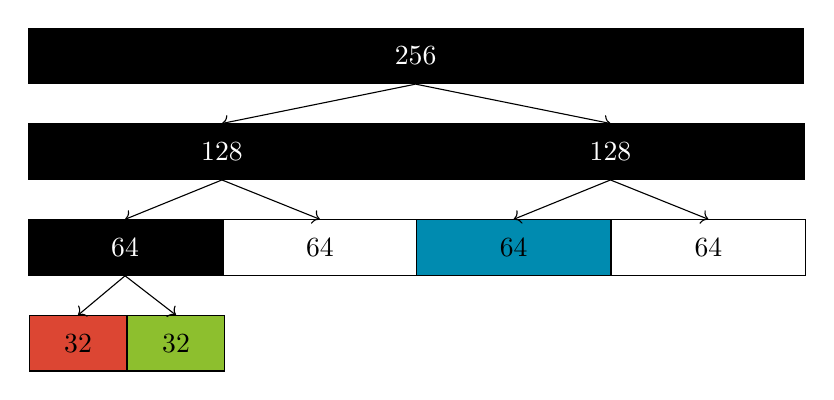
\begin{tikzpicture}[node distance=5mm and 0mm]
            
        \node[draw,rectangle,minimum width=280,minimum height=20,fill=black,text=white]    (a00)        {256};
        \node[draw,rectangle,minimum width=140,minimum height=20,fill=black,text=white,xshift=-70]    (a10) [below=of a00]       {128};
        \node[draw,rectangle,minimum width=140,minimum height=20,fill=black,text=white]    (a11) [right=of a10]       {128};
        \node[draw,rectangle,minimum width=70,minimum height=20,fill=black,text=white,xshift=-35]    (a20) [below=of a10]       {64};
        \node[draw,rectangle,minimum width=70,minimum height=20]    (a21) [right=of a20]       {64};
        \node[draw,rectangle,minimum width=70,minimum height=20,fill=pantone633,xshift=-35]    (a22) [below=of a11]       {64};
        \node[draw,rectangle,minimum width=70,minimum height=20]    (a23) [right=of a22]       {64};
        \node[draw,rectangle,minimum width=35,minimum height=20,fill=pantonewarmred,xshift=-17]    (a30) [below=of a20]       {32};
        \node[draw,rectangle,minimum width=35,minimum height=20,fill=pantone376]    (a31) [right=of a30]       {32};

        \draw[->] (a00.south) -- (a10.north);
        \draw[->] (a00.south) -- (a11.north);
        \draw[->] (a10.south) -- (a20.north);
        \draw[->] (a10.south) -- (a21.north);
        \draw[->] (a11.south) -- (a22.north);
        \draw[->] (a11.south) -- (a23.north);
        \draw[->] (a20.south) -- (a30.north);
        \draw[->] (a20.south) -- (a31.north);

    \end{tikzpicture}
    \medskip

    Where do we allocate a request of size 32?

  \end{slide}

  \begin{slide}
    
    \slidetitle{Using the Buddy Allocator (3)}

    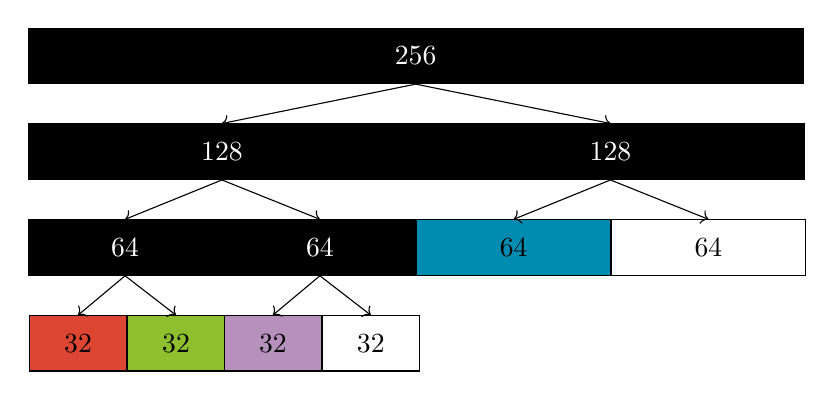
\begin{tikzpicture}[node distance=5mm and 0mm]
            
        \node[draw,rectangle,minimum width=280,minimum height=20,fill=black,text=white]    (a00)        {256};
        \node[draw,rectangle,minimum width=140,minimum height=20,fill=black,text=white,xshift=-70]    (a10) [below=of a00]       {128};
        \node[draw,rectangle,minimum width=140,minimum height=20,fill=black,text=white]    (a11) [right=of a10]       {128};
        \node[draw,rectangle,minimum width=70,minimum height=20,fill=black,text=white,xshift=-35]    (a20) [below=of a10]       {64};
        \node[draw,rectangle,minimum width=70,minimum height=20,fill=black,text=white]    (a21) [right=of a20]       {64};
        \node[draw,rectangle,minimum width=70,minimum height=20,fill=pantone633,xshift=-35]    (a22) [below=of a11]       {64};
        \node[draw,rectangle,minimum width=70,minimum height=20]    (a23) [right=of a22]       {64};
        \node[draw,rectangle,minimum width=35,minimum height=20,fill=pantonewarmred,xshift=-17]    (a30) [below=of a20]       {32};
        \node[draw,rectangle,minimum width=35,minimum height=20,fill=pantone376]    (a31) [right=of a30]  {32};
        \node[draw,rectangle,minimum width=35,minimum height=20,fill=pantone2613!50,xshift=-17]    (a32) [below=of a21]       {32};
        \node[draw,rectangle,minimum width=35,minimum height=20,]    (a33) [right=of a32]       {32};

        \draw[->] (a00.south) -- (a10.north);
        \draw[->] (a00.south) -- (a11.north);
        \draw[->] (a10.south) -- (a20.north);
        \draw[->] (a10.south) -- (a21.north);
        \draw[->] (a11.south) -- (a22.north);
        \draw[->] (a11.south) -- (a23.north);
        \draw[->] (a20.south) -- (a30.north);
        \draw[->] (a20.south) -- (a31.north);
        \draw[->] (a21.south) -- (a32.north);
        \draw[->] (a21.south) -- (a33.north);

    \end{tikzpicture}
    \medskip

    What happens when we free the size 64 block?

\end{slide}

\begin{slide}
  
  \slidetitle{Using the Buddy Allocator (4)}

  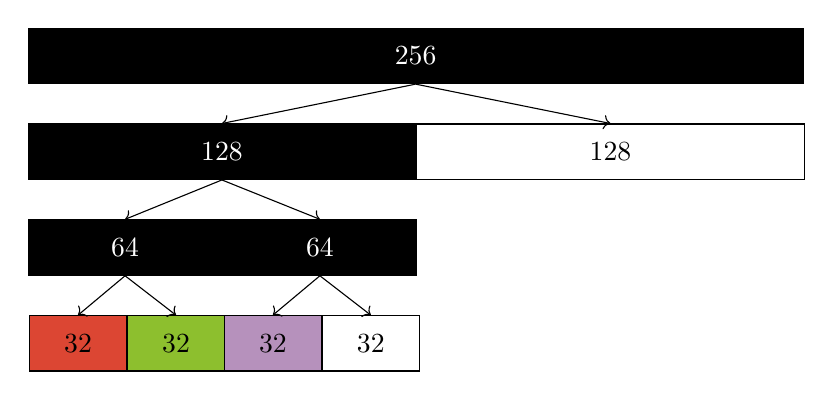
\begin{tikzpicture}[node distance=5mm and 0mm]
          
      \node[draw,rectangle,minimum width=280,minimum height=20,fill=black,text=white]    (a00)        {256};
      \node[draw,rectangle,minimum width=140,minimum height=20,fill=black,text=white,xshift=-70]    (a10) [below=of a00]       {128};
      \node[draw,rectangle,minimum width=140,minimum height=20]    (a11) [right=of a10]       {128};
      \node[draw,rectangle,minimum width=70,minimum height=20,fill=black,text=white,xshift=-35]    (a20) [below=of a10]       {64};
      \node[draw,rectangle,minimum width=70,minimum height=20,fill=black,text=white]    (a21) [right=of a20]       {64};
      \node[draw,rectangle,minimum width=35,minimum height=20,fill=pantonewarmred,xshift=-17]    (a30) [below=of a20]       {32};
      \node[draw,rectangle,minimum width=35,minimum height=20,fill=pantone376]    (a31) [right=of a30]  {32};
      \node[draw,rectangle,minimum width=35,minimum height=20,fill=pantone2613!50,xshift=-17]    (a32) [below=of a21]       {32};
      \node[draw,rectangle,minimum width=35,minimum height=20,]    (a33) [right=of a32]       {32};

      \draw[->] (a00.south) -- (a10.north);
      \draw[->] (a00.south) -- (a11.north);
      \draw[->] (a10.south) -- (a20.north);
      \draw[->] (a10.south) -- (a21.north);
      \draw[->] (a20.south) -- (a30.north);
      \draw[->] (a20.south) -- (a31.north);
      \draw[->] (a21.south) -- (a32.north);
      \draw[->] (a21.south) -- (a33.north);

  \end{tikzpicture}

\end{slide}

\begin{slide}

  \slidetitle{Buddy Allocators are Used in Linux}

  Advantages

  \leftspace{}Fast and simple compared to general dynamic memory allocation

  \leftspace{}Avoids external fragmentation by keeping free physical pages contiguous
  \medskip

  Disadvantages

  \leftspace{}There's always internal fragmentation

  \leftspace{}\leftspace{}We always round up the allocation size if it's not a
  power of 2

\end{slide}

\begin{slide}
  
  \slidetitle{Slab Allocators Take Advantage of Fixed Size Allocations}

  Allocate objects of same size from a dedicated pool

  \leftspace{}All structures of the same type are the same size
  \medskip

  Every object type has it's own pool with blocks of the correct size

  \leftspace{}This prevents internal fragmentation

\end{slide}

\begin{slide}

  \slidetitle{Slab is a Cache of ``Slots''}

  Each allocation size has a corresponding slab of slots
  
  (one slot holds one allocation)
  \medskip

  Instead of a linked list, we can use a bitmap
  
  (there's a mapping between bit and slot)

  \leftspace{}For allocations, we set the bit and return the slot

  \leftspace{}For deallocations, we just clear the bit
  \medskip

  The slab can be implemented on top of the buddy allocator

\end{slide}

\begin{slide}
  
  \slidetitle{Each Slab Can Be Allocated using the Buddy Allocator}
  
  Consider two object sizes: A and B
  \medskip
  
  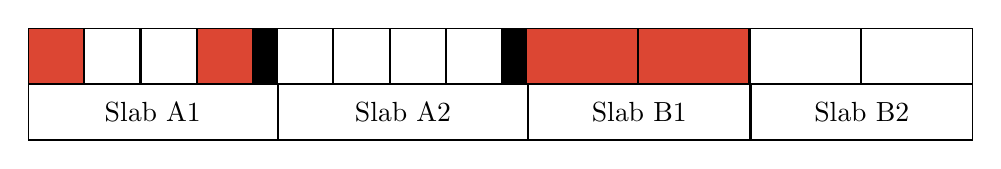
\begin{tikzpicture}[node distance=0mm and 0mm]

      \node[draw,rectangle,minimum width=20,minimum height=20,fill=pantonewarmred]    (a0)        {};
      \node[draw,rectangle,minimum width=20,minimum height=20]    (a1)     [right=of a0]   {};
      \node[draw,rectangle,minimum width=20,minimum height=20]    (a2)     [right=of a1]   {};
      \node[draw,rectangle,minimum width=20,minimum height=20,fill=pantonewarmred]    (a3)     [right=of a2]   {};
      \node[draw,rectangle,minimum width=8,minimum height=20,fill=black]    (a4)     [right=of a3]   {};

      \node[draw,rectangle,minimum width=20,minimum height=20]    (a5)     [right=of a4]   {};
      \node[draw,rectangle,minimum width=20,minimum height=20]    (a6)     [right=of a5]   {};
      \node[draw,rectangle,minimum width=20,minimum height=20]    (a7)     [right=of a6]   {};
      \node[draw,rectangle,minimum width=20,minimum height=20]    (a8)     [right=of a7]   {};
      \node[draw,rectangle,minimum width=8,minimum height=20,fill=black]    (a9)     [right=of a8]   {};


      \node[draw,rectangle,minimum width=40,minimum height=20,fill=pantonewarmred]    (b1)     [right=of a9]   {};
      \node[draw,rectangle,minimum width=40,minimum height=20,fill=pantonewarmred]    (b2)     [right=of b1]   {};

      \node[draw,rectangle,minimum width=40,minimum height=20]    (b3)     [right=of b2]   {};
      \node[draw,rectangle,minimum width=40,minimum height=20]    (b4)     [right=of b3]   {};

      \node[draw,rectangle,minimum width=90,minimum height=20,xshift=35]    (s0)    [below=of a0]   {Slab A1};
      \node[draw,rectangle,minimum width=90,minimum height=20]    (s1)    [right=of s0]   {Slab A2};
      \node[draw,rectangle,minimum width=80,minimum height=20]    (s2)    [right=of s1]   {Slab B1};
      \node[draw,rectangle,minimum width=80,minimum height=20]    (s3)    [right=of s2]   {Slab B2};

  \end{tikzpicture}
  \medskip

  We can reduce internal fragmentation if Slabs are located
  adjacently

  \leftspace{}In this example A has internal fragmentation (dark box)

\end{slide}

\begin{slide}
  
  \slidetitle{Journaling Filesystem}

  Deleting a file on a Unix file system involves three steps:

  \begin{enumerate}
    \item Removing its directory entry.
    \item Releasing the inode to the pool of free inodes.
    \item Returning all disk blocks to the pool of free disk blocks.
  \end{enumerate}
  \medskip

  Crashes could occur between any steps, leading to a storage leak
  \medskip

  The journal contains operations in progress, so if a crash occurs we can
  recover

\end{slide}

\begin{slide}

  \slidetitle{Even More Memory Allocations}

  The kernel restricts the problem for better memory allocation
  implementations

  \begin{itemize}
    \item Buddy allocator is a real-world restricted implementation
    \item Slab allocator takes advantage of fixed sized objects to reduce
          fragmentation
  \end{itemize}

\end{slide}

\end{document}
